\documentclass[12pt,letterpaper]{article}
\usepackage[utf8]{inputenc}
\usepackage{geometry}
\usepackage{graphicx}
\usepackage{hyperref}
\usepackage{amsmath}
\usepackage{setspace}
\usepackage{titlesec}
\usepackage{lmodern}
\usepackage{float}

\geometry{margin=1in}
\setstretch{1.2}

% Title formatting
\titleformat{\section}{\large\bfseries}{\thesection}{1em}{}
\titleformat{\subsection}{\normalsize\bfseries}{\thesubsection}{1em}{}

% Title page
\title{
    \vspace{2cm}
    \textbf{Project 1: Frog Tail}\\
    \vspace{0.5cm}
    \large Data analysis to understand tail regeneration.\\
    \vspace{1cm}
}
\author{
    Elias Ludviksson \\
    STATGR5243 - Applied Data Science \\
    Columbia University \\
    \vspace{0.5cm}
    \today
}
\date{}

\begin{document}

\maketitle
\newpage

\begin{abstract}
This project analyzes single-cell RNA sequencing data from Xenopus laevis tadpole tails to identify Regeneration-Organizing Cells (ROCs). The analysis pipeline, implemented using Scanpy, includes quality control, normalization, and feature selection. We compared Louvain and Leiden clustering algorithms, finding that Leiden provided superior performance across multiple metrics. Cluster enrichment analysis successfully identified a cluster (Leiden cluster 11) corresponding to the known ROC population. Differential gene expression analysis was performed to identify marker genes for this cluster. We evaluated the impact of two data correction techniques: denoising by regressing out cell cycle effects and batch integration by regressing out sample batch effects. Results showed that denoising significantly improved clustering accuracy (ARI from 0.582 to 0.685) and dramatically increased the recovery of established ROC marker genes from 10.2\% to 28.6\%. Batch integration also offered improvements, though less pronounced. These findings demonstrate a complete analysis workflow and highlight the critical role of accounting for technical and biological covariates in scRNA-seq analysis.
\end{abstract}

\newpage
\setcounter{page}{1}
\tableofcontents
\newpage

\section{Introduction}

Some Xenopus laevis tadpoles have tails which can regenerate after amputation. The tails of these tadpoles contain a variety of cell types, including muscle cells, skin cells, and spinal cord cells.
A study by C. Aztekin et al. found the regeneration-organizing cells (ROCs) in the tadpole tails, which are crucial for tail regeneration. They performed single-cell RNA sequencing on these tadpoles to study the gene expression profiles of different cell types during tail regeneration.
The dataset is publicly available \href{https://ftp.ebi.ac.uk/biostudies/fire/E-MTAB-/716/E-MTAB-7716/Files/arrayExpressUpload.zip}{online}. To learn the clustering and gene analysis techniques used on single-cell genomic data, we will analyze this dataset using scanpy, scikit-learn, pandas, and numpy.

\section{Methods}
The data is in an AnnData format containing 13,199 cells × 31,535 genes. The entire analysis workflow was implemented using the Scanpy library in Python.

\subsection{Quality Control and Normalization}
Initial quality control involved filtering out cells with fewer than 100 genes and genes expressed in fewer than 10 cells. We then used Scanpy's implementation of scrublet to identify and remove potential doublets. For downstream analysis, the data was normalized to the median total counts per cell and then log-transformed. We selected the top 2000 highly variable genes for computational efficiency.

\subsection{Dimensionality Reduction and Clustering}
We performed Principal Component Analysis (PCA) on the normalized data, retaining the top 50 principal components. A k-nearest neighbors (k-NN) graph was computed from these components, which served as the basis for clustering. We compared the Louvain and Leiden community detection algorithms. The resulting clusters were visualized using UMAP. Performance was evaluated using the Rand index, Adjusted Rand Index (ARI), Silhouette Score, and Mutual Information against the known cell type labels.

\subsection{Cluster Enrichment Analysis}
To identify the ROC cluster, we focused on cells present at day 0 post-amputation. We performed a Fisher's exact test on each Leiden cluster to find those statistically enriched with cells from day 0. This list was further filtered for cells in the 'st40' developmental stage and 'G1' cell cycle phase, which pinpointed cluster 11 as the putative ROC cluster.

\subsection{Gene Expression Analysis}
Using the Wilcoxon rank-sum test and a t-test, we identified the top 40 differentially expressed genes for cluster 11. These marker gene lists were compared against the known ROC genes from Supplementary Table 3 of the source publication.

\subsection{Denoising and Batch Integration}
We evaluated two techniques to correct for unwanted variation in the data:
\begin{enumerate}
    \item \textbf{Denoising:} We used \text{sc.pp.regress\_out} to remove the confounding effect of the cell cycle by treating \verb|CellCyclePhase| as a covariate.
    \item \textbf{Batch Integration:} We used \text{sc.pp.regress\_out} to correct for technical variability between experimental batches, using the \texttt{batch} annotation as a covariate.
\end{enumerate}
The impact of these steps was assessed by re-running the clustering and marker selection pipelines and comparing the quantitative metrics to the original, uncorrected analysis.

\subsection{Code Availability}
The code for this project is publicly available at: \\
\url{https://colab.research.google.com/drive/1HZrv7ODnstypcYvlFyD7D5xdXL_oS01C#scrollTo=71a41724}\\
\url{https://github.com/Skatturinn/ADS_H1_FROG}

\section{Results}
\subsection{Clustering Analysis}
Leiden clustering consistently outperformed Louvain across all metrics, achieving a higher ARI (0.582 vs. 0.553) and Silhouette Score (0.330 vs. 0.317). Therefore, Leiden was used for all subsequent analyses.

\begin{figure}[H]
    \centering
    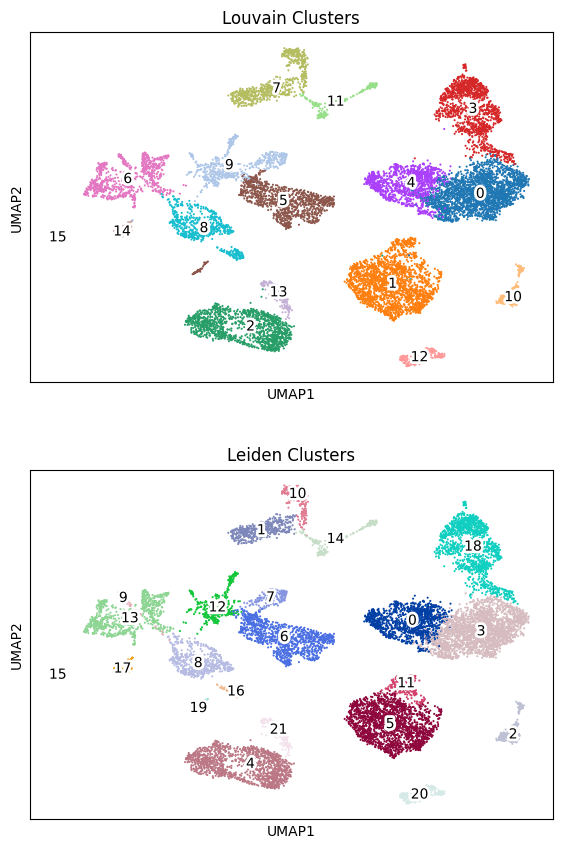
\includegraphics[width=0.8\textwidth]{figures/leiden_louvain_clusters.png}
    \caption{UMAP visualization comparing Leiden and Louvain clustering results against known cell type annotations.}
    \label{fig:clustering}
\end{figure}

\subsection{Impact of Denoising and Batch Integration}
Enrichment analysis successfully identified Leiden cluster 11 as the ROC cluster. In the original analysis, the identified marker genes for this cluster had a low overlap with the reference gene set (10.2\%).

Applying correction methods significantly improved the results. Denoising by regressing out cell cycle effects yielded the most substantial improvement, boosting the clustering ARI to 0.685 and increasing the marker gene overlap to 28.6\%. Batch integration also improved the results, with the ARI increasing to 0.591 and gene overlap reaching 14.3\%, but the effect was less pronounced. While the denoised data had the best quantitative metrics, the UMAP visualization of the integrated data appeared to show a more distinct ROC cluster.

\begin{figure}[H]
    \centering
    % Placeholder for gene expression dotplot
    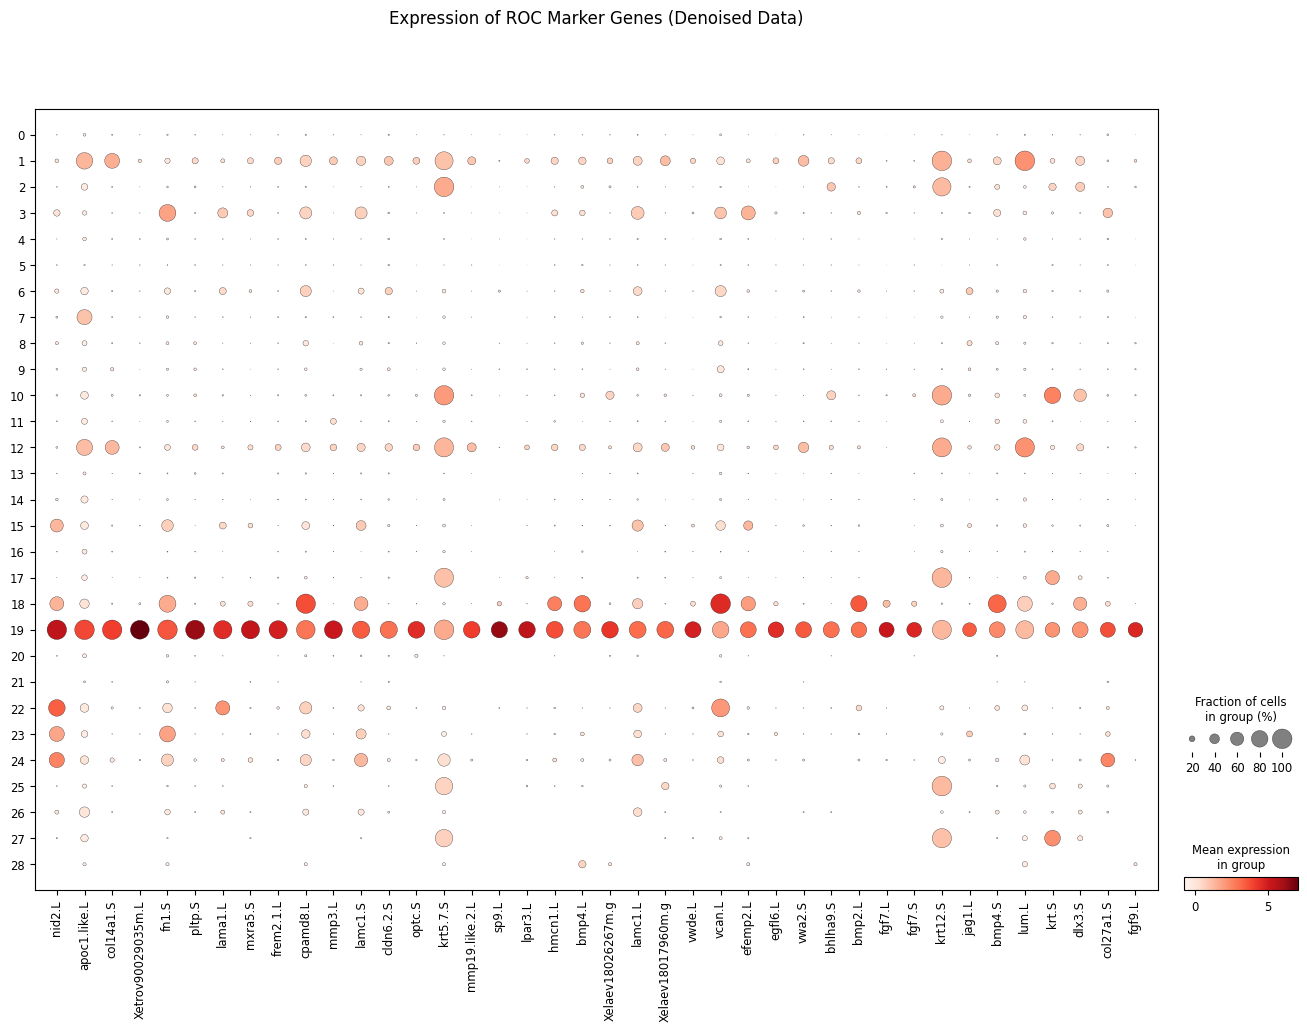
\includegraphics[width=0.9\textwidth]{figures/gene_expression_dotplot.png}
    \caption{Gene expression analysis results. This figure would typically be a dotplot showing the expression of top marker genes for the ROC cluster (Cluster 11) in the denoised data, which provided the best marker recovery.}
    \label{fig:gene_expression}
\end{figure}

\begin{table}[H]
\centering
\caption{Impact of Denoising and Integration on Clustering and Marker Identification.}
\begin{tabular}{|l|c|c|c|}
\hline
\textbf{Metric (Leiden)} & \textbf{Original} & \textbf{Denoised} & \textbf{Integrated} \\ \hline
Adjusted Rand & 0.582 & 0.685 & 0.591 \\ \hline
Silhouette & 0.330 & 0.311 & 0.222 \\ \hline
Table 3 Gene Overlap & 10.2\% & 28.6\% & 14.3\% \\ \hline
\end{tabular}
\end{table}

\section{Conclusion}
This project successfully implemented a single-cell analysis pipeline to identify a rare cell population in a complex biological dataset. Our analysis confirms that Leiden clustering is often superior to Louvain for community detection in biological networks.

Most importantly, our findings highlight the critical impact of correcting for covariates. Denoising the data by regressing out cell cycle effects led to a dramatic improvement in both clustering accuracy and, more critically, the biological relevance of the findings, as evidenced by the nearly three-fold increase in the recovery of known marker genes. Batch integration also provided a benefit, underscoring the importance of addressing technical artifacts. This demonstrates that careful preprocessing and removal of confounding variables are essential steps for extracting meaningful biological insights from scRNA-seq data.

\end{document}